% Fig. 1 -- Overview of AgriFuseNet.
% Build:  python make_fig1_assets.py   (image assets, once)
%         pdflatex fig_pipeline.tex && pdftoppm -png -r 600 -singlefile fig_pipeline.pdf fig_pipeline
\documentclass[border=3pt]{standalone}
\usepackage[T1]{fontenc}
\usepackage[scaled=0.92]{helvet}
\renewcommand{\familydefault}{\sfdefault}
\usepackage{amsmath,amssymb}
\usepackage{sansmath}
\sansmath
\usepackage{graphicx}
\usepackage{tikz}
\usetikzlibrary{positioning,arrows.meta,calc,shapes.multipart}

% ---------------------------------------------------------------- style
% black outlines and text; soft fills by block function (frozen backbone, fixed features, projection,
% attention/pooling, classifier, leaf-blade encoder)
\definecolor{ink}{HTML}{1F1F1F}
\colorlet{line}{black!80}
\definecolor{frozenfill}{HTML}{E6E6E6}
\definecolor{mlpfill}{HTML}{D6ECF3}
\definecolor{attfill}{HTML}{FBE3CC}
\definecolor{clsfill}{HTML}{F4D5DC}
\definecolor{leaffill}{HTML}{DDEFD6}
% panel (b): own fills for the trained blocks inside the leaf-blade encoder
\definecolor{bprojfill}{HTML}{D3C7EA}
\definecolor{battfill}{HTML}{FFF0BF}
\definecolor{tok}{HTML}{8C9DAF}
\colorlet{typ}{black!40}

\tikzset{
  >={Stealth[length=2.4mm,width=1.6mm,inset=0.95mm]},
  ar/.style={->,line width=0.65pt,draw=black},
  box/.style={rounded corners=2pt,line width=0.6pt,align=center,inner sep=3pt,font=\small,text=ink,draw=line},
  frozen/.style={box,fill=frozenfill},
  fixed/.style={box,fill=white},
  att/.style={box,fill=attfill},
  clsb/.style={box,fill=clsfill},
  leafenc/.style={box,fill=leaffill},
  head/.style={font=\normalsize\bfseries,text=ink,anchor=base},
  note/.style={font=\footnotesize,text=ink!75,align=center},
  lab/.style={font=\footnotesize,text=ink},
  img/.style={inner sep=0pt,draw=ink!35,line width=0.3pt},
  plus/.style={circle,draw=black,line width=0.6pt,minimum size=3.8mm,inner sep=0pt,fill=white,font=\small},
  % two-compartment encoder: frozen backbone | trained projection
  split enc/.style={rectangle split,rectangle split horizontal,rectangle split parts=2,
    rectangle split part fill={frozenfill,mlpfill},draw=line,line width=0.6pt,rounded corners=2pt,
    font=\small,text=ink,inner sep=3pt,minimum height=0.85cm,align=center},
}
% horizontal vector: \hvec{x0}{y}{n}{colour}{cell}
\newcommand{\hvec}[5]{\foreach \i in {1,...,#3}{\filldraw[fill=#4,draw=white,line width=0.4pt] ($(#1,#2)+(\i*#5-#5,-#5/2)$) rectangle +(#5,#5);}}
% vertical vector: \vvec{x}{y0}{n}{colour}{cell}, cells hang down from y0
\newcommand{\vvec}[5]{\foreach \i in {1,...,#3}{\filldraw[fill=#4,draw=white,line width=0.4pt] ($(#1,#2)+(-#5/2,-\i*#5)$) rectangle +(#5,#5);}}

\begin{document}
\begin{tikzpicture}[x=1cm,y=1cm]

% grid: rows and column centres (gaps between neighbouring blocks >= 0.45 cm)
\def\rA{6.3} \def\rB{4.5} \def\rC{2.7} \def\rD{0.9}
\def\xRaw{0.95} \def\xSam{3.35} \def\xCrop{5.65} \def\xEnc{7.95} \def\xPlus{9.7}
\def\xTok{10.25} \def\xPool{13.35} \def\xCls{15.55} \def\xOut{16.65}
\def\imgw{1.35}
\def\yhead{7.8} \def\ybot{-0.42}
% tall blocks (SAM 3, fusion) share the same top and bottom edges
\def\tallc{3.72} \def\tallh{7.5cm}

% ================================================================ (a)
\node[font=\normalsize\bfseries,text=ink,anchor=base west] at (-0.8,\yhead) {(a)};
\foreach \y/\org/\lab in {\rA/leafwidth/Leaf blade, \rB/leavePattern/Leaf top, \rC/buddataset/Bud, \rD/crossSection/Cross-section}{
  \node[img] (raw-\org) at (\xRaw,\y) {\includegraphics[width=\imgw cm]{assets/raw_\org.png}};
  \node[font=\small,text=ink,rotate=90] at (-0.12,\y) {\lab};
}
\node[head] at (\xRaw,\yhead) {Specimen};

% SAM 3 (frozen) with one prompt box per organ: identical size, centred on the row
\node[frozen,minimum width=2.4cm,minimum height=\tallh] (sam) at (\xSam,\tallc) {};
\node[font=\small\bfseries,text=ink] at (\xSam,7.08) {SAM 3 \textmd{(frozen)}};
\foreach \y/\p in {\rA/{\mbox{long narrow leaf}\\\mbox{grass blade}},\rB/{\mbox{plant}\\\mbox{sugarcane leaf}},\rC/{\mbox{sugarcane stalk}},\rD/{\mbox{food, slice}}}{
  \node[fixed,font=\footnotesize\itshape,text width=1.98cm,minimum height=0.8cm,inner sep=2.5pt] at (\xSam,\y) {\p};
}
\node[head] at (\xSam,\yhead) {Segmentation};
\node[note,anchor=north] at (\xSam,-0.15) {concept\\prompts};
\foreach \y/\org in {\rA/leafwidth,\rB/leavePattern,\rC/buddataset,\rD/crossSection}{
  \draw[ar] (raw-\org.east) -- (sam.west |- 0,\y);
  \node[img] (crop-\org) at (\xCrop,\y) {\includegraphics[width=\imgw cm]{assets/crop_\org.png}};
  \draw[ar] (sam.east |- 0,\y) -- (crop-\org.west);
}
\node[head] at (\xCrop,\yhead) {Crop};
\node[note,anchor=north] at (\xCrop,-0.15) {background\\removed};

% organ encoders
\node[leafenc,minimum width=2.25cm,minimum height=0.85cm] (E1) at (\xEnc,\rA) {Leaf-blade\\encoder (b)};
\foreach \y/\k/\org in {\rB/2/leavePattern,\rC/3/buddataset,\rD/4/crossSection}{
  \node[split enc] (E\k) at (\xEnc,\y) {\makebox[1.12cm]{DINOv2}\nodepart{two}\makebox[0.62cm]{MLP}};
  \draw[ar] (crop-\org.east) -- (E\k.west);
}
\node[head] at (\xEnc,\yhead) {Encoder $E_o$};
\draw[ar] (crop-leafwidth.east) -- (E1.west);

% organ-type embeddings and organ tokens
\foreach \y/\k in {\rA/1,\rB/2,\rC/3,\rD/4}{
  \node[plus] (p\k) at (\xPlus,\y) {$+$};
  \draw[ar] (E\k.east) -- (p\k.west);
  \hvec{\xPlus-0.36}{\y+0.72}{3}{typ}{0.24}
  \node[lab,anchor=west] at (\xPlus+0.4,\y+0.72) {$\mathbf{e}_\k$};
  \draw[ar] (\xPlus,\y+0.6) -- (p\k.north);
}
\foreach \y/\k in {\rA/1,\rB/2,\rD/4}{
  \hvec{\xTok}{\y}{6}{tok}{0.26}
  \draw[ar] (p\k.east) -- (\xTok-0.05,\y);
}
% organ removed by organ dropout
\foreach \i in {1,...,6}{\draw[black!40,dashed,line width=0.4pt,fill=white] (\xTok+\i*0.26-0.26,\rC-0.13) rectangle +(0.26,0.26);}
\draw[ar] (p3.east) -- (\xTok-0.05,\rC);
\node[note,anchor=north] at (\xTok+0.78,\rC-0.24) {organ dropout};
\node[head] at (\xTok+0.78,\yhead) {Token $\mathbf{t}_o$};

% organ-set pooling
\node[att,minimum width=2.2cm,minimum height=\tallh] (pool) at (\xPool,\tallc) {};
\node[font=\small\bfseries,text=ink,align=center] at (\xPool,6.92) {Masked\\mean};
\node[font=\small,text=ink] at (\xPool,3.6) {$\mathbf{s}=\dfrac{\sum_o m_o\,\mathbf{t}_o}{\sum_o m_o}$};
\node[note] at (\xPool,1.55) {any subset\\of organs};
\foreach \y in {\rA,\rB,\rC,\rD}{\draw[ar] (\xTok+1.62,\y) -- (pool.west |- 0,\y);}
\node[head] at (\xPool,\yhead) {Fusion};

% classifier and output
% classifier drawn as a trapezoid (128-D specimen code -> 5 variety scores); 'cls' gives the anchors
\node[inner sep=0pt,minimum width=1.35cm,minimum height=1.95cm] (cls) at (\xCls,3.6) {};
\filldraw[fill=clsfill,draw=line,line width=0.6pt,rounded corners=2pt]
  (cls.north west) -- ($(cls.north east)+(0,-0.32)$) -- ($(cls.south east)+(0,0.32)$) -- (cls.south west) -- cycle;
\node[font=\small,text=ink,align=center] at (cls.center) {LN\\Linear\\softmax};
\draw[ar] (pool.east |- 0,3.6) -- node[above=3.5pt,pos=0.42,lab]{$\mathbf{s}$} (cls.west);
\foreach \i/\v/\w/\c in {0/CP77-400/0.12/black!25, 1/CPF-237/0.95/black!65, 2/CPF-250/0.20/black!25, 3/CPF-251/0.08/black!25, 4/CPF-253/0.14/black!25}{
  \fill[\c] (\xOut+0.15,4.55-\i*0.47) rectangle +(\w*1.05,0.26);
  \node[lab,anchor=west] at (\xOut+0.2+\w*1.05,4.68-\i*0.47) {\v};
}
\draw[ar] (cls.east) -- (\xOut+0.05,3.6);
\node[head] at (\xOut+1.0,\yhead) {Variety};

% ================================================================ (b) leaf-blade encoder
\def\yb{-1.05}
\draw[black!35,line width=0.5pt] (-0.8,\yb+0.05) -- (18.95,\yb+0.05);
\node[font=\normalsize\bfseries,text=ink,anchor=base west] at (-0.8,\yb-0.5) {(b)};
\node[font=\normalsize\bfseries,text=ink,anchor=base west] at (-0.15,\yb-0.5) {Leaf-blade encoder $E_1$};

% three equally spaced branch rows; the middle one is the centre line of the projection and attention blocks
\def\yB{-2.4} \def\yT{-3.75} \def\yH{-5.1} \def\yM{-3.75}
% inputs
\node[img] (mb) at (0.65,\yB) {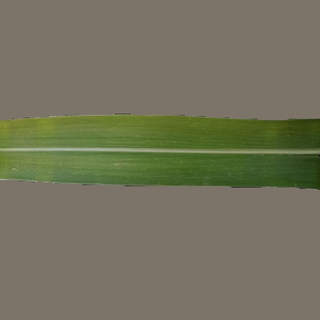
\includegraphics[width=1.15cm]{assets/blade_masked.png}};
\node[note,anchor=north] at (mb.south) {masked blade};
\node[img] (band) at (1.5,\yH) {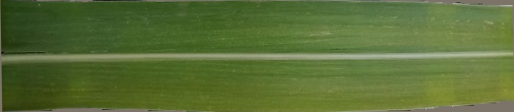
\includegraphics[width=2.95cm]{assets/blade_band.png}};
\node[note,anchor=north] at (band.south) {rectified blade};
\def\xDino{4.15}
\foreach \k in {0,1,2,3}{\node[img] (tile\k) at (\xDino-1.02+\k*0.68,\yT) {\includegraphics[width=0.58cm]{assets/tile_\k.png}};}
\node[note,anchor=north] at (\xDino,\yT-0.31) {blade tiles};
\draw[ar] (band.north -| 2.0,0) |- (tile0.west);

% branches
\node[frozen,minimum width=2.0cm,minimum height=0.6cm] (dino) at (\xDino,\yB) {DINOv2};
\draw[ar] (mb.east) -- (dino.west);
\draw[ar] (\xDino,\yT+0.3) -- (dino.south);
% branch vectors start at \xv; arrows into and out of the vectors have the same length \arl
\def\xv{9.0} \def\arl{0.62}
\node[fixed,minimum width=3.85cm,minimum height=0.95cm,anchor=east] (bot) at (\xv-0.08-\arl,\yH) {botanical descriptors (164-D)\\[-1pt]{\footnotesize colour, texture, venation, shape}};
\draw[ar] (band.east) -- (bot.west);

\foreach \y/\lab in {\yB/{\mathbf{f}_{\mathrm{blade}}}, \yT/{\mathbf{f}_{\mathrm{tile}}}, \yH/{\mathbf{f}_{\mathrm{bot}}}}{
  \hvec{\xv}{\y}{4}{black!45}{0.24}
  \node[lab,anchor=south] at (\xv+0.48,\y+0.13) {$\lab$};
}
\draw[ar] (dino.east) -- (\xv-0.08,\yB);
\draw[ar] (dino.east) ++(1.0,0) |- (\xv-0.08,\yT);
\node[note,anchor=south] at (7.7,\yT+0.02) {tile mean};
\draw[ar] (bot.east) -- (\xv-0.08,\yH);

% projections and channel-wise attention
% projection drawn as an encoder trapezoid (taller input side, shorter output side); the invisible node
% 'proj' gives the anchors used by the arrows
\def\projh{3.7cm} \def\taper{0.32}
\node[inner sep=0pt,minimum width=1.5cm,minimum height=\projh,anchor=west] (proj) at (\xv+0.96+0.06+\arl,\yM) {};
\filldraw[fill=bprojfill,draw=line,line width=0.6pt,rounded corners=2pt]
  (proj.north west) -- ($(proj.north east)+(0,-\taper)$) -- ($(proj.south east)+(0,\taper)$) -- (proj.south west) -- cycle;
\node[font=\small,text=ink,align=center] at (proj.center) {LN\\Dropout\\MLP};
\foreach \y in {\yB,\yT,\yH}{\draw[ar] (\xv+1.02,\y) -- (proj.west |- 0,\y);}
\node[box,fill=battfill,minimum width=3.85cm,minimum height=\projh,anchor=west] (caf) at ($(proj.east)+(\arl,0)$) {};
\node[font=\small\bfseries,text=ink,align=center] at (caf.center |- 0,\yB) {Channel-wise attention};
\node[font=\small,text=ink] at ($(caf.center)+(0,0.33)$) {$a_{b,j}=\operatorname{softmax}_b\, G_{b,j}$};
\node[font=\small,text=ink] at ($(caf.center)+(0,-0.33)$) {$\mathbf{z}_{\mathrm{leaf}}=\textstyle\sum_b \mathbf{a}_b\odot\mathbf{u}_b$};
\node[note] at (caf.center |- 0,\yH) {modality dropout};
\foreach \y in {\yB,\yT,\yH}{\draw[ar] (proj.east |- 0,\y) -- (caf.west |- 0,\y);}
\node[lab,anchor=south] at ($(proj.east |- 0,\yB)+(\arl*0.42,0.1)$) {$\mathbf{u}_b$};
% z_leaf one arrow length after the attention block (caf.east = \xv + 1.02 + 3*\arl... evaluated below)
\path (caf.east) ++(\arl+0.12,0) coordinate (zc);
\path let \p1=(zc) in node[lab,anchor=south] at (\x1,\yM+0.6) {$\mathbf{z}_{\mathrm{leaf}}$};
\path let \p1=(zc) in coordinate (ztop) at (\x1,\yM+0.6);
\foreach \i in {1,...,5}{\filldraw[fill=tok,draw=white,line width=0.4pt] ($(ztop)+(-0.12,-\i*0.24)$) rectangle +(0.24,0.24);}
\draw[ar] (caf.east) -- ++(\arl,0);
\node[note,anchor=west,align=left] at ($(zc)+(0.35,0)$) {output of $E_1$\\in (a)};

\end{tikzpicture}
\end{document}
